%======================================================================
% SANDRA ECOSYSTEM - Diseño Revista Editorial Premium (Mejorado)
%======================================================================

\documentclass[11pt, spanish, letterpaper, openany]{book}

\usepackage{fontspec}
\setmainfont{Inter}[Path = assets/fonts/, Extension = .otf, UprightFont = *-Regular, BoldFont = *-Bold]
\setsansfont{Inter}[Path = assets/fonts/, Extension = .otf, UprightFont = *-Medium]

\usepackage[
    top=2cm,
    bottom=2.5cm,
    left=2cm,
    right=2cm,
    columnsep=16pt
]{geometry}

\usepackage{graphicx}
\usepackage{wrapfig}
\usepackage{fancyhdr}
\usepackage{titlesec}
\usepackage{xcolor}
\usepackage{microtype}
\usepackage{tikz}
\usetikzlibrary{calc}
\usepackage[most]{tcolorbox}
\usepackage{fontawesome5}
\usepackage{parskip}
\usepackage{booktabs}
\usepackage{setspace}

%--------------------------------------------------------------------
% COLORES
%--------------------------------------------------------------------
\definecolor{sandraDark}{HTML}{1A2634}
\definecolor{sandraTeal}{HTML}{00897B}
\definecolor{sandraGold}{HTML}{FF8F00}
\definecolor{sandraLight}{HTML}{E0F2F1}
\definecolor{sandraCream}{HTML}{FAFAFA}
\definecolor{sandraGray}{HTML}{90A4AE}
\definecolor{sandraText}{HTML}{455A64}
\definecolor{isoBlue}{HTML}{1565C0}
\definecolor{isoGreen}{HTML}{2E7D32}
\definecolor{isoOrange}{HTML}{EF6C00}
\definecolor{isoAmber}{HTML}{FFF8E1}

%--------------------------------------------------------------------
% INTERLINEADO Y ESPACIADO
%--------------------------------------------------------------------
\setstretch{1.4}
\setlength{\parskip}{0.8ex}
\setlength\partopsep{0pt}

%--------------------------------------------------------------------
% CABECERA SIMPLE
%--------------------------------------------------------------------
\pagestyle{fancy}
\fancyhf{}
\fancyhead[RO]{\rightmark}
\fancyhead[LE]{\leftmark}
\fancyfoot[CO]{\thepage}
\fancyfoot[RO,LE]{\color{sandraGray}\fontsize{7}{9}\selectfont\itshape Sandra Ecosystem}

\addtolength{\headheight}{14pt}

%--------------------------------------------------------------------
% BANNER DE CAPÍTULO
%--------------------------------------------------------------------
\newcommand{\chapterbanner}[1]{
\thispagestyle{empty}
\begin{tikzpicture}[remember picture, overlay]
    \fill[sandraDark] (current page.north west) -- (current page.north east) -- (current page.south east) -- (current page.south west) -- cycle;
    \fill[sandraGold] ([xshift=0pt] current page.north west) rectangle ([xshift=5mm] current page.south west);
    \node[anchor=south east] at ([xshift=-1cm, yshift=1cm] current page.south east) {
        {\fontsize{120}{130}\selectfont\bfseries\color{white!10}#1}
    };
    \node[anchor=west] at ([xshift=1.2cm, yshift=-2.5cm] current page.north west) {
        \parbox{0.6\linewidth}{
            \fontsize{32}{38}\selectfont\bfseries\color{white}#1
        }
    };
    \fill[sandraTeal] (current page.north west) rectangle ([xshift=5mm, yshift=-3mm] current page.north west);
\end{tikzpicture}
\clearpage
}

\titleformat{\section}{\normalfont\large\bfseries\color{sandraDark}}{\thesection}{0.5em}{}
\titlespacing*{\section}{0pt}{1.5ex plus 0.5ex}{0.5ex}

%--------------------------------------------------------------------
% CAJAS PEQUEÑAS Y LIMPIAS
%--------------------------------------------------------------------
\newtcolorbox{notaeditorial}{
    colback=sandraCream,
    colframe=sandraTeal,
    boxrule=0.5pt,
    left=4pt,
    right=4pt,
    top=4pt,
    bottom=4pt,
    before skip=6pt,
    after skip=6pt
}

\newtcolorbox{estandarISO}{
    colback=sandraLight,
    colframe=isoBlue,
    boxrule=0.5pt,
    rounded corners,
    before skip=6pt,
    after skip=6pt
}

\newtcolorbox{alertaISO}{
    colback=isoAmber,
    colframe=isoOrange,
    boxrule=0.5pt,
    rounded corners,
    before skip=6pt,
    after skip=6pt
}

%--------------------------------------------------------------------
% DROP CAP ELEGANTE
%--------------------------------------------------------------------
\usepackage{lettrine}
\lettrinefont{\fontsize{32}{36}\selectfont\bfseries\color{sandraDark}}
\lettrineafterlen=2pt
\lettrinelinenums=false

%--------------------------------------------------------------------
% SEPARADOR
%--------------------------------------------------------------------
\newcommand{\separador}{
    \vspace{0.5ex}
    \begin{center}
        \color{sandraTeal}\rule{0.15\linewidth}{0.5pt}
    \end{center}
    \vspace{0.5ex}
}

%--------------------------------------------------------------------
% IMAGEN LATERAL PEQUEÑA
%--------------------------------------------------------------------
\newenvironment{imagentexto}{
\begin{wrapfigure}{O}{0.42\linewidth}
    \centering
    \vspace{-4pt}
}{
    \vspace{4pt}
\end{wrapfigure}
}

\usepackage[spanish]{babel}

\begin{document}

%======================================================================
% CAPÍTULO 2: MARCO TEÓRICO
%======================================================================
\chapterbanner{02}

\section{Estado del Arte}

\lettrine{E}{l} middleware empresarial ha evolucionado significativamente hasta convertirse en plataformas complejas de integración. El mercado ofrece soluciones como IBM Integration Bus, MuleSoft, Apache Camel y Spring Integration.

\begin{imagentexto}
    
\includegraphics[width=\linewidth]{assets/mockup/golang.png}
    \caption{Go: rendimiento y concurrencia}
\end{imagentexto}

Sin embargo, la mayoría fueron diseñadas para mercados desarrollados, ignorando necesidades específicas de regiones con infraestructura limitada.

\begin{notaeditorial}
    \textbf{Nota del Autor}: El desarrollo de middleware propio representa una oportunidad estratégica para garantizar la soberanía tecnológica.
\end{notaeditorial}

\separador

\section{Fundamentos de Middleware}

El middleware actúa como puente entre aplicaciones y el sistema operativo. Un Enterprise Service Bus (ESB) representa la evolución hacia arquitectura basada en servicios.

\begin{estandarISO}
    \textbf{ESB en Sandra}: Implementado en Go para alto rendimiento y miles de conexiones simultáneas.
\end{estandarISO}

Características principales:
\begin{itemize}
    \item Transformación de mensajes entre formatos
    \item Enrutamiento basado en reglas
    \item Composición de servicios
    \item Transacciones distribuidas
\end{itemize}

\separador

\section{Arquitectura de Microservicios}

Servicios pequeños, autónomos y débilmente acoplados. Cada microservicio es responsable de una funcionalidad específica.

\begin{imagentexto}
    
\includegraphics[width=\linewidth]{assets/mockup/rust.png}
    \caption{Rust: seguridad de memoria}
\end{imagentexto}

El ecosistema Sandra:
\begin{itemize}
    \item \textbf{Server}: Middleware central
    \item \textbf{Consola}: Interfaz web
    \item \textbf{SDC}: Aplicación de escritorio
    \item \textbf{Sentinel}: Procesamiento de eventos
\end{itemize}

\separador

\section{Modelo Zero Trust}

Elimina la confianza implícita, verificando cada solicitud independientemente de su origen.

\begin{imagentexto}
    
\includegraphics[width=\linewidth]{assets/mockup/angular.png}
    \caption{Angular: frontend enterprise}
\end{imagentexto}

\begin{estandarISO}
    \textbf{ISO 27001}: Sistema de Gestión de Seguridad
\end{estandarISO}

Principios fundamentales:
\begin{enumerate}
    \item \textbf{Verificación explícita}: Autenticación MFA
    \item \textbf{Mínimo privilegio}: Permisos mínimos
    \item \textbf{Verificación continua}: Monitoreo
\end{enumerate}

\begin{alertaISO}
    \textbf{Consideración}: Zero Trust requiere cambio cultural organizacional.
\end{alertaISO}

\separador

\section{Tecnologías del Ecosistema}

\begin{imagentexto}
    
\includegraphics[width=\linewidth]{assets/mockup/tauri.png}
    \caption{Tauri: escritorio ligero}
\end{imagentexto}

Tecnologías de última generación:

\begin{tabular}{lp{4.5cm}}
    \textbf{Go 1.24} & Rendimiento y concurrencia \\
    \textbf{Rust} & Seguridad de memoria \\
    \textbf{Angular} & Frontend enterprise \\
    \textbf{Tauri} & Aplicaciones de escritorio \\
    \textbf{gRPC} & Comunicación entre servicios \\
    \textbf{WebSockets} & Tiempo real \\
\end{tabular}

\begin{notaeditorial}
    \textbf{Nota Técnica}: Go + Tauri proporciona equilibrio óptimo.
\end{notaeditorial}

\clearpage

%======================================================================
% CAPÍTULO 3: MARCO LEGAL
%======================================================================
\chapterbanner{03}

\section{Ley de Infogobierno}

\lettrine{L}{a} Ley de Infogobierno establece normas para el uso de tecnologías en el sector público venezolano, promoviendo Soberanía Tecnológica y Software Libre.

\begin{imagentexto}
    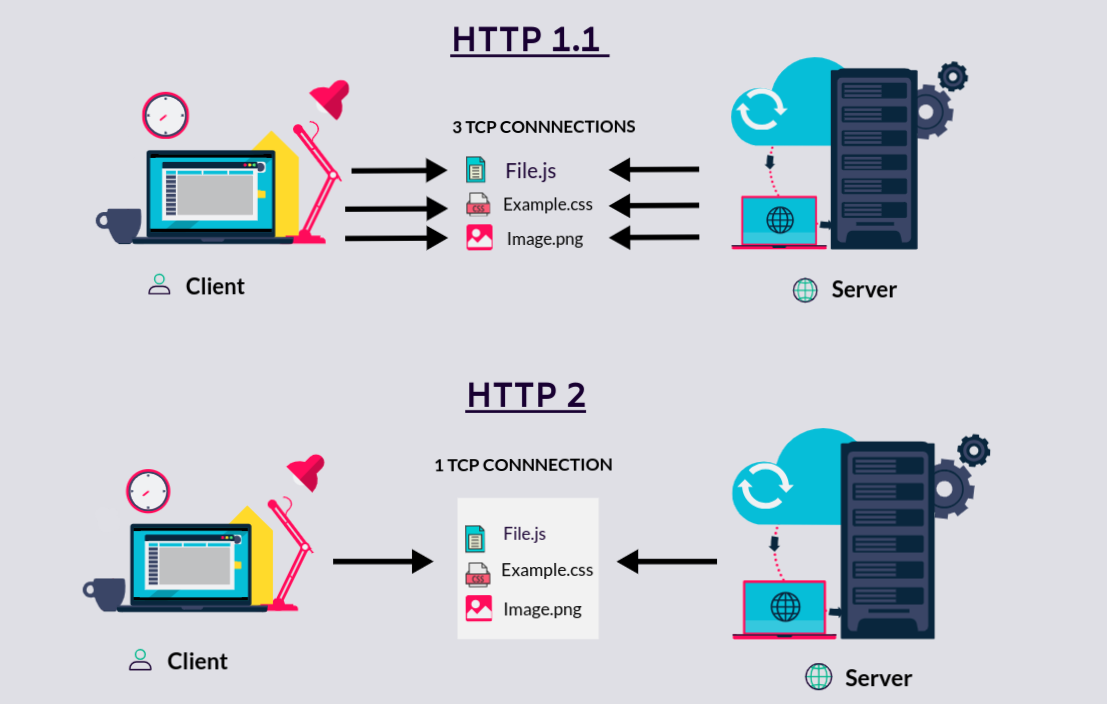
\includegraphics[width=\linewidth]{assets/mockup/http1-http2.png}
    \caption{Protocolos HTTP}
\end{imagentexto}

\begin{table}
    \centering
    \small
    \caption{Cumplimiento Ley de Infogobierno}
    \begin{tabular}{lp{4.5cm}}
        \toprule
        \textbf{Requisito} & \textbf{Implementación} \\
        \midrule
        Software Libre & Código abierto \\
        Estándares Abiertos & REST, gRPC, JSON \\
        Interoperabilidad & APIs documentadas \\
        Seguridad & AES-256, JWT, MFA, TLS \\
        \bottomrule
    \end{tabular}
\end{table}

\separador

\section{Delitos Informáticos}

Controles para prevenir conductas penalizadas:

\begin{imagentexto}
    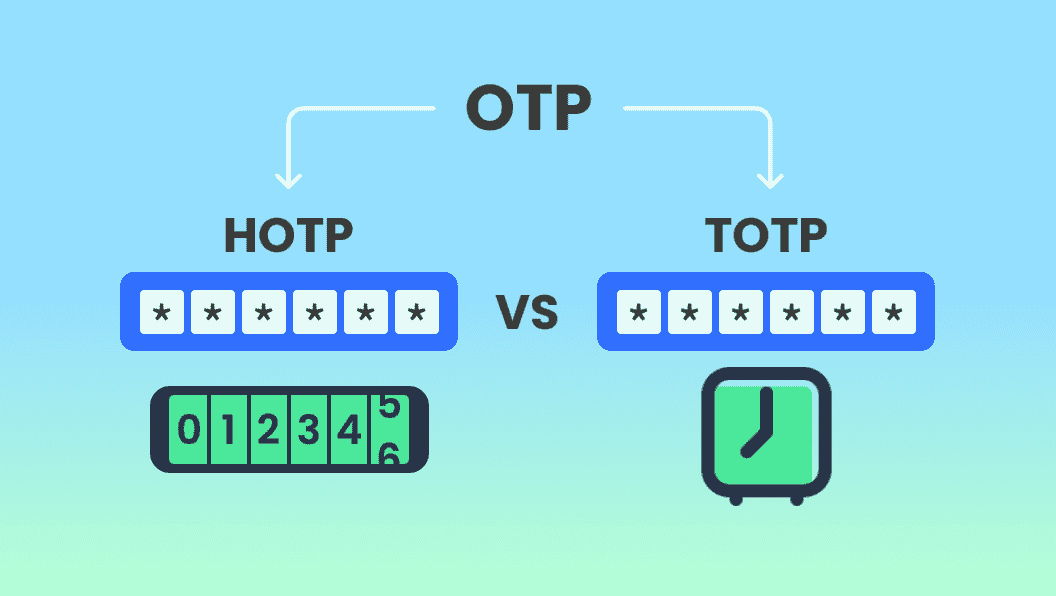
\includegraphics[width=\linewidth]{assets/mockup/otp-hotp-totp.png}
    \caption{Autenticación multifactor}
\end{imagentexto}

\begin{itemize}
    \item \textbf{Acceso no autorizado}: MFA
    \item \textbf{Interceptación}: Cifrado en tránsito y reposo
    \item \textbf{Falsificación}: Firmas digitales y logs
    \item \textbf{Destrucción}: Sistemas de backup
\end{itemize}

\separador

\section{Estándares Internacionales}

\begin{estandarISO}
    \textbf{ISO/IEC 27001}: Gestión de Seguridad de la Información
\end{estandarISO}

\begin{estandarISO}
    \textbf{ISO/IEC 27002}: 93 controles de seguridad
\end{estandarISO}

\begin{estandarISO}
    \textbf{NIST SP 800-53}: Controles de seguridad y privacidad
\end{estandarISO}

\separador

\section{Licenciamiento Soberano}

\begin{imagentexto}
    
\includegraphics[width=\linewidth]{assets/mockup/workflow.png}
    \caption{Workflow de seguridad}
\end{imagentexto}

La elección de licencias es estratégica para garantizar autonomía tecnológica.

\begin{alertaISO}
    \textbf{Nota Estratégica}: Licencias permisivas (Apache 2.0, MIT) permiten privatizar innovaciones.
\end{alertaISO}

\begin{table}
    \centering
    \small
    \caption{Análisis de licenciamiento}
    \begin{tabular}{lp{4.5cm}}
        \toprule
        \textbf{Licencia} & \textbf{Implicación} \\
        \midrule
        Apache 2.0 / MIT & Permite clasificar módulos \\
        GPL v3 / AGPL & Copyleft prohíbe cierre \\
        \bottomrule
    \end{tabular}
\end{table}

\begin{notaeditorial}
    \textbf{Nota Final}: El licenciamiento estratégico es crucial para entornos de defensa.
\end{notaeditorial}

\end{document}
